\section{Qualitative results}
\label{sec:qualitative}

\subsection{Overall}

Looking at examples that are well-predicted by our approach in Fig \ref{fig:qualitative} (1b, 2b, 3b), it demonstrates good segmentation masks with clear and smooth mask boundaries. Some small organs can also be seen segmented successfully and precisely meaning that both proposed modules can work effectively with organs having various sizes. For reference, we use \cite{py06itksnap} for all the CT volume visualization in our project.

\begin{figure}[!h]
\centering
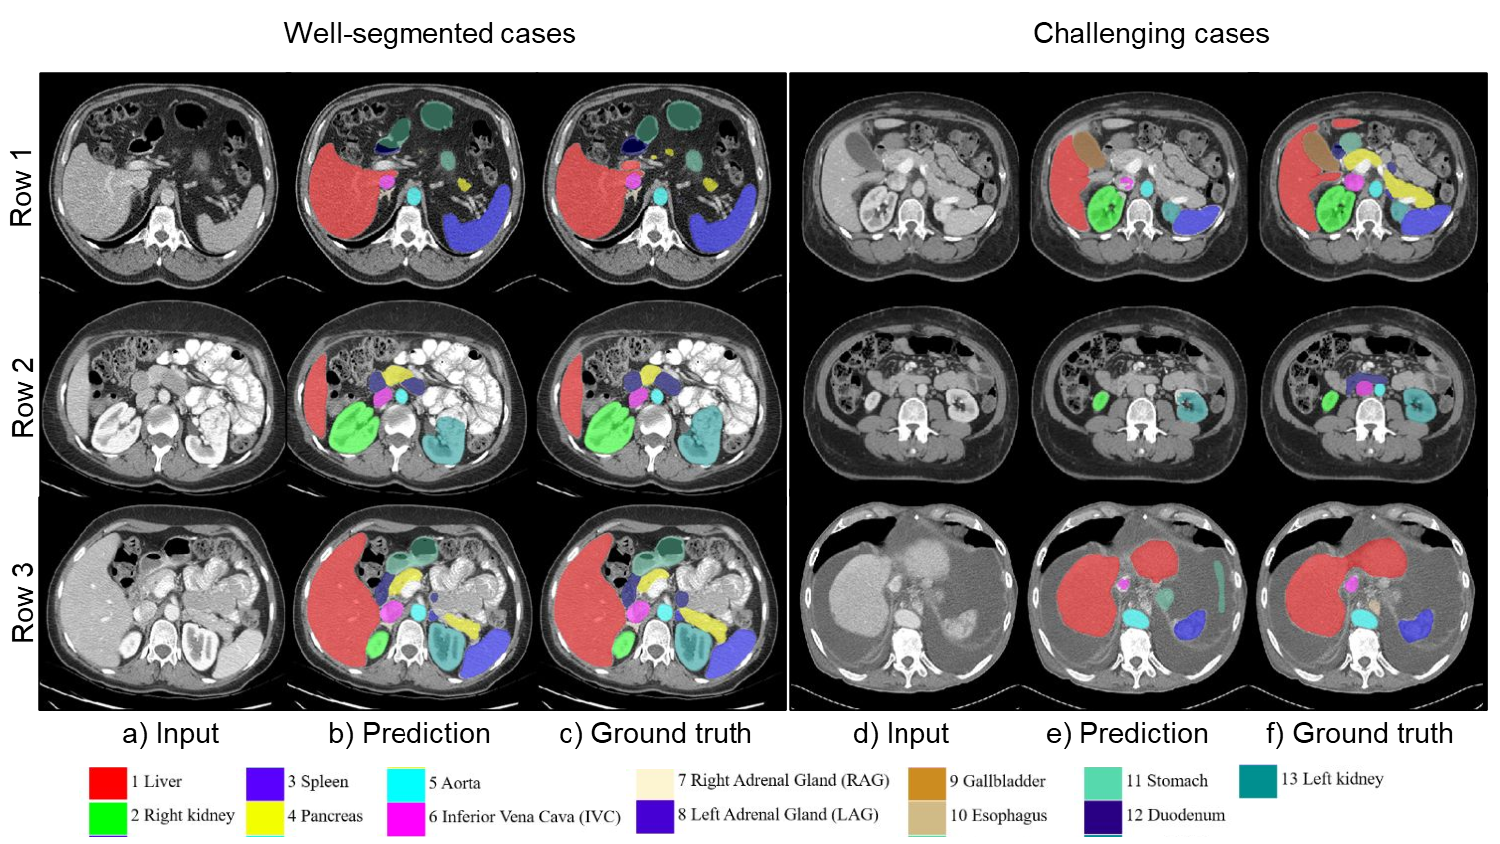
\includegraphics[width=\textwidth]{content/resources/new_images/qualitative.pdf}
\caption{Qualitative results from the validation set. We illustrate both well-segmented and challenging examples for our proposed segmentation pipeline}
\label{fig:qualitative}
\end{figure}

On the other hand, our models suffer from various difficult cases where organs are missing. Generally, there are two cases that negatively affect our approach:

\begin{enumerate}
    \item Relatively small organs (adrenal glands (Fig \ref{fig:qualitative} (1e)), gallbladder (Fig \ref{fig:qualitative} (1e)), and esophagus (Fig \ref{fig:qualitative} (3e))) account for the lowest DSC since they usually are failed to be identified by the Reference module.
    \item Other organs (pancreas (Fig \ref{fig:qualitative} (1e)) and duodenum (Fig \ref{fig:qualitative} (2e))) despite having a larger size, yet their lengths on the axial plane are short and sometimes occluded by many surrounding organs, which can affect how the information propagating through the slices, causing class confusion in the result. 
\end{enumerate}

Furthermore, due to our two-staged pipeline, for the results of the second stage to be good really relies on the first stage's performance.  If the reference stage miss-segments any organ, that one will be missed during the entire propagation process. Having said that, this issue mostly just occurs in organs that have a short-size length on the axial plane.  


\subsection{Improvement of Mask Propagation}

\begin{figure}[!h]
\centering
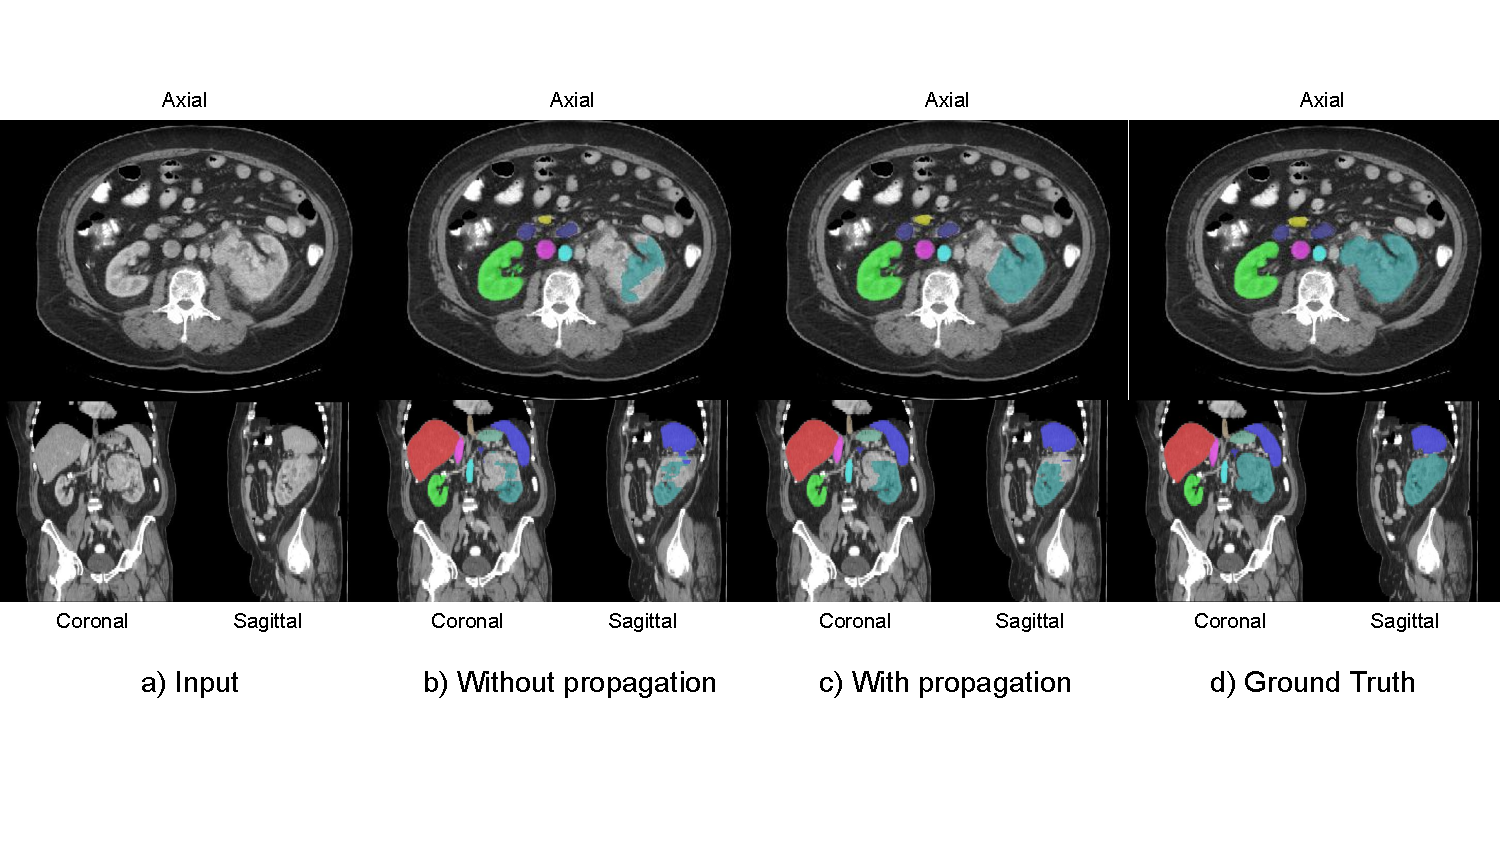
\includegraphics[width=\textwidth]{content/resources/new_images/qualitative/stcn_improvement.pdf}
\caption{Qualitative comparison between before and after mask-propagated refinement.}
\label{fig:stcn}
\end{figure}

\begin{figure}[!h]
\centering
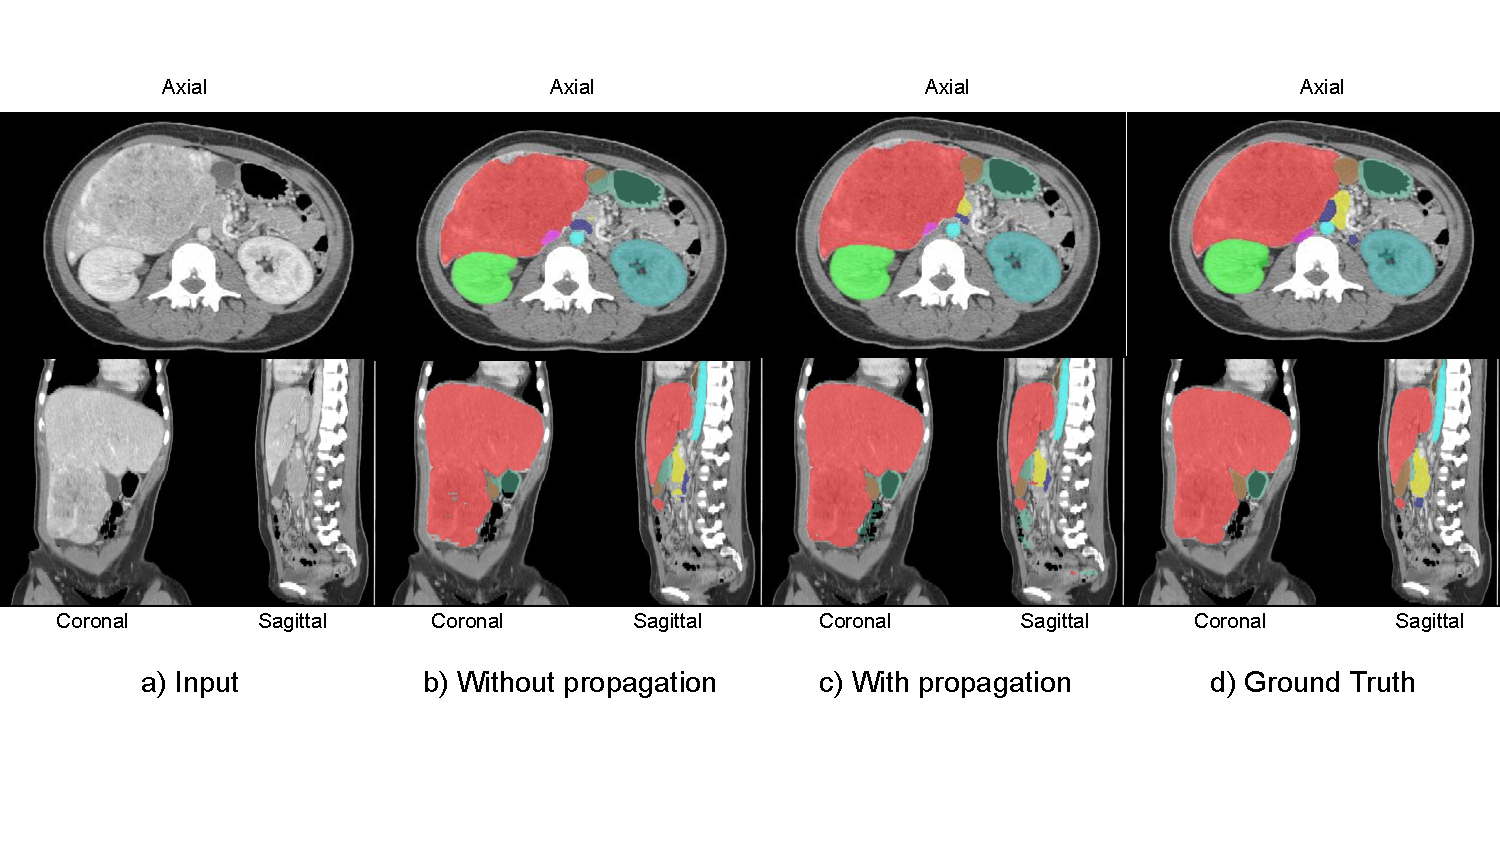
\includegraphics[width=\textwidth]{content/resources/new_images/qualitative/stcn_improvement2.pdf}
\caption{Another qualitative comparison between before and after mask-propagated refinement }
\label{fig:stcn2}
\end{figure}

Figure \ref{fig:stcn} and Figure \ref{fig:stcn2} showcases the refinement results of our proposed Propagation module. It can be recognized that the "Without propagation" columns represent the output masks of the Reference stage only.  We can see that with the second stage applied, some organ masks become smoother and more precise along the coronal and sagittal axis (the left kidney in Figure \ref{fig:stcn} and both the gallbladder, pancreas in Figure \ref{fig:stcn2}).

While the masks from the first stage are usually inconsistent along the temporal dimension, even between two consecutive frames, the Mask Propagation algorithm helps to stabilize the differences between them.

\subsection{Improvement of Cross Pseudo Supervision}

\begin{figure}[!h]
\centering
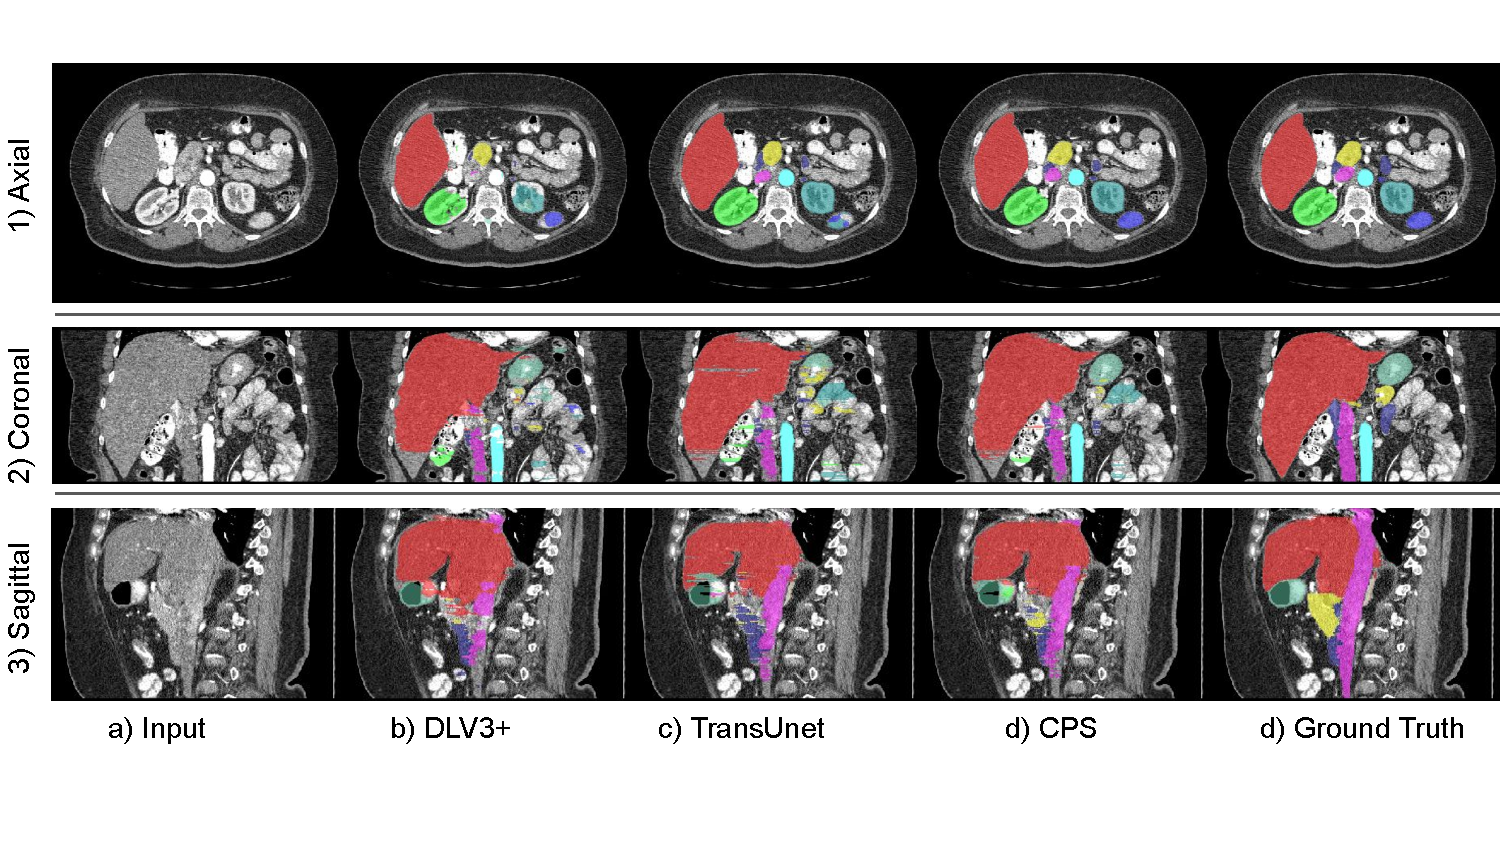
\includegraphics[width=\textwidth]{content/resources/new_images/qualitative/cps.pdf}
\caption{Comparison between before and after using Cross Pseudo Supervision in the Reference stage}
\label{fig:cps_improvement}
\end{figure}

The effectiveness of using CPS can be seen in Figure \ref{fig:cps_improvement}. It seems that the DeeplabV3+ and the TransUnet suffer from segmenting some different specific organs with small areas. CPS, on the other hand, gives more stable results (the small part of the spleen in the bottom right in the axial view, or the reduction in inconsistency along the sagittal plane, both in Figure \ref{fig:cps_improvement}).

\subsection{Improvement of Positional Encoding}

\begin{figure}[!h]
\centering
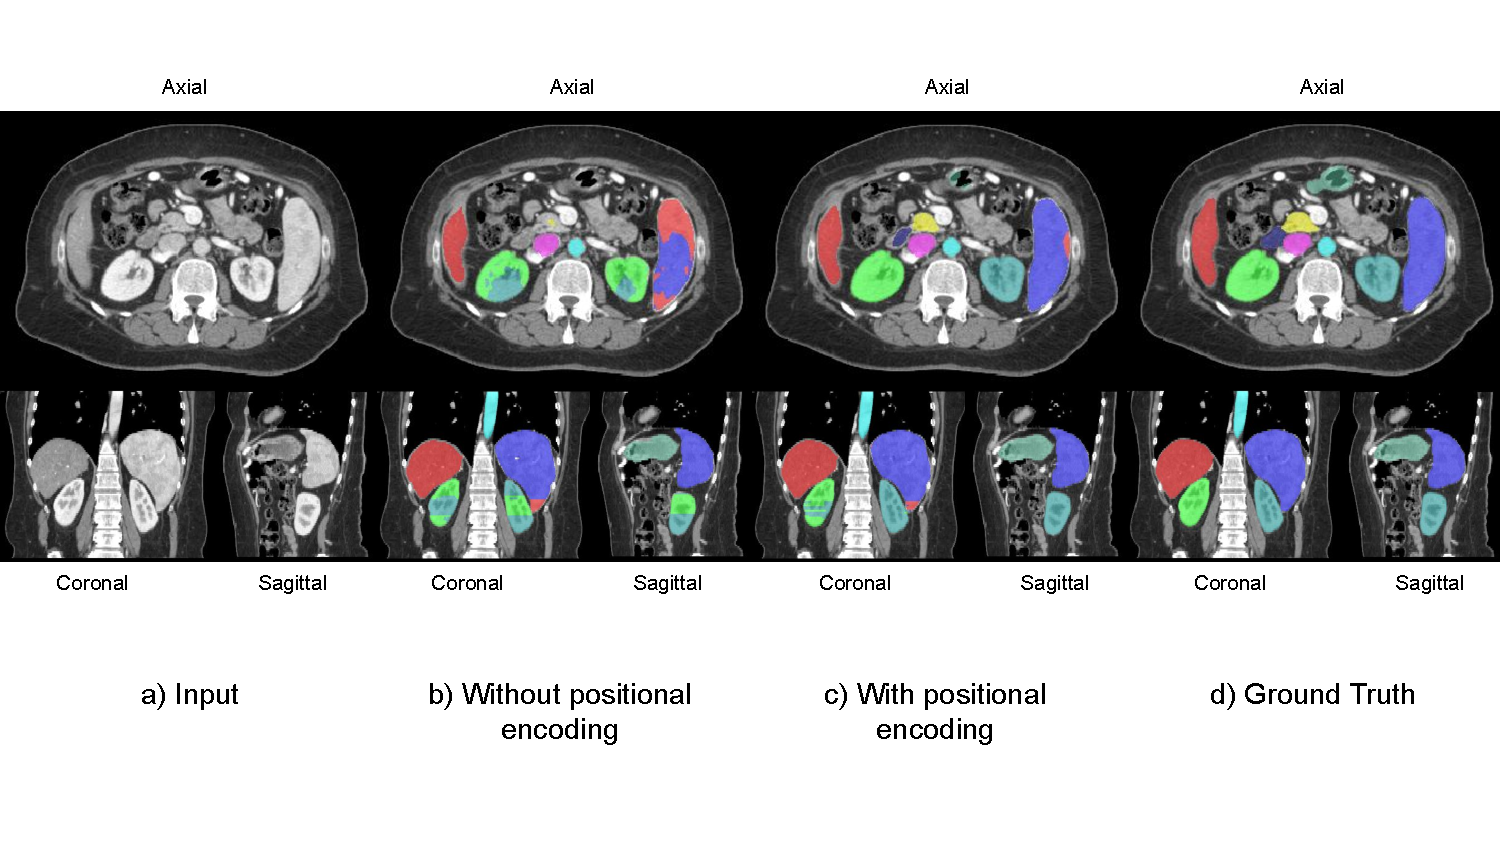
\includegraphics[width=\textwidth]{content/resources/new_images/qualitative/positional_encoding.pdf}
\caption{Comparison between before and after integrating positional encoding into the TransUnet in the Reference stage}
\label{fig:pe_improvement}
\end{figure}

The positional encoding includes the temporal information in the input of the Reference module. Therefore, it is expected to reduce the discordance between the sequence of slices. For example, the right kidney in Figure \ref{fig:pe_improvement} b), viewed in coronal and sagittal, is constantly mistaken for the right kidney. With the introduction of positional information, it is segmented accordingly. Moreover, it also accurately identifies the location of the pancreas and the left adrenal gland.


\subsection{Improvement of Pseudo Labeling with Uncertainty Estimation}

\begin{figure}[!h]
\centering
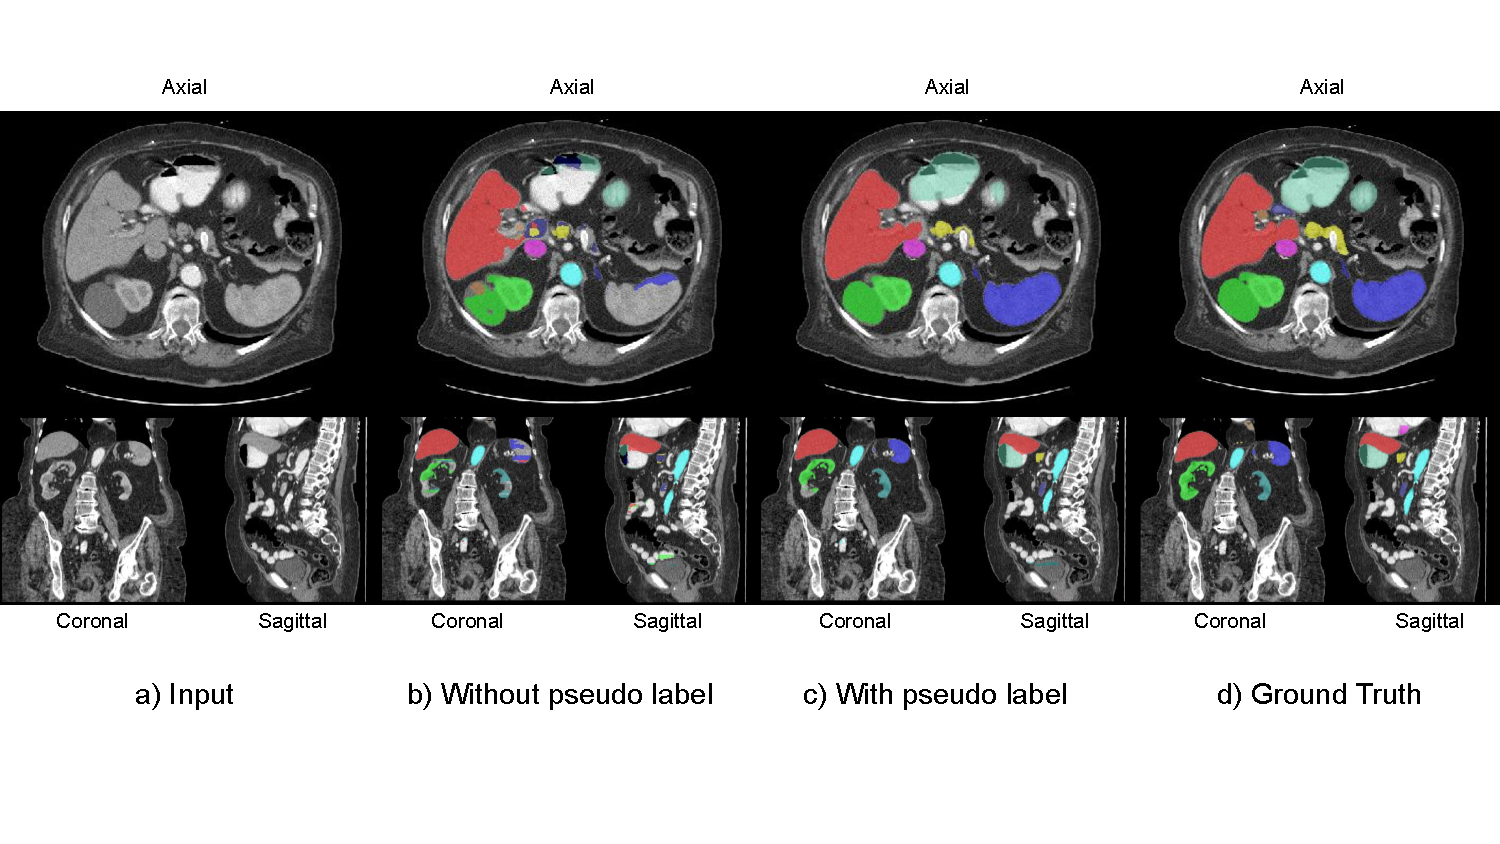
\includegraphics[width=\textwidth]{content/resources/new_images/qualitative/pseudo_labeling.pdf}
\caption{Comparison between before using pseudo labeling and after retraining the model with pseudo labeling}
\label{fig:pseudo_labeling_improvement}
\end{figure}

It is clear that the contribution of pseudo-labeling is significant to our final results. In Figure \ref{fig:pseudo_labeling_improvement}, most of the organ masks are notably enhanced after retraining with pseudo labels. However, we still have yet to resolve the imbalanced problem, which leads to the difficulty in identifying small organs like the gallbladder in the Figure. 